%%%%%%%%%%%%%%%%%%%%%%%%%%%%%%%%%%%%%%
\documentclass[a4paper,english]{report}    % list options between brackets


\RequirePackage{color}
\RequirePackage{float}
\RequirePackage{amsfonts}
\RequirePackage{amsmath}
\RequirePackage{alltt}
\RequirePackage{ae}
\RequirePackage{times}
\RequirePackage{fancyhdr}
\RequirePackage{graphicx} 
\RequirePackage{makeidx}  
\RequirePackage{wrapfig}

\RequirePackage{hyperref}

\UseRawInputEncoding

\hypersetup{
    bookmarks=true,         % show bookmarks bar?
    unicode=false,          % non-Latin characters in Acrobat�s bookmarks
    pdftoolbar=true,        % show Acrobat�s toolbar?
    pdfmenubar=true,        % show Acrobat�s menu?
    pdffitwindow=false,     % window fit to page when opened
    pdfstartview={Fit},    % fits the width of the page to the window
    pdftitle={Elmer GUI Tutorials},    % title
    pdfauthor={CSC - IT Center for Science},     % author
    pageanchor=true,
    hyperindex=true,
    pdfnewwindow=true,      % links in new window
    colorlinks=true,       % false: boxed links; true: colored links
    linkcolor=black,          % color of internal links
    citecolor=black,        % color of links to bibliography
    filecolor=black,      % color of file links
    urlcolor=black           % color of external links
}
 
\renewcommand{\vec}[1]{\mathbf{#1}} 
 
\makeindex             
  

\newcommand{\menu}[2]{{\it \vskip2mm #1 $\rightarrow$ #2 \vskip2mm}}
\newcommand{\dynmenu}[3]{{\it \vskip2mm #1 $\rightarrow$ #2 $\rightarrow$ #3 \vskip2mm}}


% Use these to make the printable area bigger
% Also have the option 'ownsize' active in the documentclass
\setlength{\hoffset}{-15mm}
\setlength{\voffset}{-10mm}
\addtolength{\textwidth}{30mm}
\addtolength{\textheight}{20mm}
%\addtolength{\headwidth}{30mm}


% Command file syntax stuff
\definecolor{SifCol}{rgb}{0.5,0.5,0.5}
%\definecolor{SifCol}{rgb}{1,1,1}

% Index for keywords
\newcommand{\sifitem}[2]{\item[\tt{#1}]\index{#1}\hspace{1mm}{\color{SifCol}\hspace{1mm}\tt{#2}}\newline} 
%item with two fields but no text
\newcommand{\sifitemnt}[2]{\item[\tt{#1}]\index{#1}\hspace{1mm}{\color{SifCol}\hspace{1mm}\tt{#2}}} 


\newcommand{\sifbegin}{\begin{description}}
\newcommand{\sifend}{\end{description}}
\newcommand{\modinfo}[2]{{\bf{#1}}: {#2}\newline}

\newcommand{\ttbegin}{\begin{alltt}}
\newcommand{\ttend}{\end{alltt}}
\newcommand{\keno}{$\backslash$}


\newcommand{\Sf}[1]{\textsf{#1}}
\newcommand{\Bf}[1]{{\sffamily\bfseries}}

\newcommand{\URL}[1]{\texttt{#1}}

% Some new commands...
\def\xwin{X Window System}
\def\xbr{Xbrowse}
\def\prag{\Tt{\#pragma}}

\newcommand{\inxgra}[2]{{\centerline{\includegraphics[width=#1]{#2}}}}
\newcommand{\inygra}[2]{{\centerline{\includegraphics[height=#1]{#2}}}}
\newcommand{\incgra}[2]{{\centerline{\includegraphics[height=#1]{#2}}}}

\providecommand{\ftn}{Fort\-ran~90}
\providecommand{\Idx}[1]{{#1}\index{#1}}


%%%%%%%%%%%%%%%% Math definitions for Elmer Solver Manuals %%%%%%%%%%%%%%%%%
\newcommand{\Bfm}[1]{\mbox{\boldmath{${#1}$}}}

\newcommand{\tensorspace}[1]{\boldsymbol{#1}}         % Sets of tensors are bold italic
\newcommand{\tensor}[1]{\boldsymbol{#1}}              % Tensors are bold italic
\newcommand{\point}[1]{\mathbf{#1}}                   % Points are bold upright
\newcommand{\pointf}[1]{\mathbf{#1}}                  % Point-valued functions are bold upright
\newcommand{\pointfm}[1]{\mbox{\boldmath{${#1}$}}}    % Point-valued functions for math symbols

\DeclareMathOperator{\grad}{\mathbf{grad}}            % The spatial gradient operator
\newcommand{\Grad}{\mbox{\boldmath{${\nabla}$}}}      % gradient with respect to the points of the reference configuration
\DeclareMathOperator{\curl}{\mathbf{curl}}            % The spatial curl operator
\DeclareMathOperator{\Curl}{\mathbf{Curl}}            % curl with respect to the points of the reference configuration
\DeclareMathOperator{\rot}{\mathbf{rot}}              % rot operator defined for scalars
\DeclareMathOperator{\divs}{\mathrm{div}}             % scalar-valued divergence
\DeclareMathOperator{\divvec}{\mathbf{div}}           % vector-valued divergence
\DeclareMathOperator{\Divvec}{\mathbf{Div}}           % vector-valued divergence w. r. t. the points of the reference configuration
\newcommand{\Div}{\nabla\cdot}                        

%\newcommand{\Vec}[1]{\vec{#1}}
%\newcommand{\Vec}[1]{\mathify{\mathbf{#1}}}

%\newcommand{\Matr}[1]{\mbox{${#1}$}}                  % Matrices are just italic to differentiate between true tensors and matrices
\newcommand{\Matr}[1]{{#1}}                     % Matrices
\newcommand{\Der}[2]{\frac{\partial{#1}}{\partial{#2}}}
\newcommand{\Secder}[2]{\frac{\partial^2{#1}}{\partial{#2}^2}}
\newcommand{\Inv}[1] {\frac{1}{#1}}


% Make the headings fancier
\pagestyle{fancy}

\lhead[\normalfont\small\bf\thepage]{\normalfont\small\slshape\rightmark}
\rhead[\small\slshape\lefthead]{\normalfont\small\bf \thepage}
%\setlength{\headrulewidth}{0.4pt}
%\renewcommand{\chaptermark}[1]{\markright{\bf \chaptername \ \thechapter.\ #1}{}}
\renewcommand{\chaptermark}[1]{\markright{\bf \thechapter.\ #1}{}}
\renewcommand{\sectionmark}[1]{}
\renewcommand{\subsectionmark}[1]{}
\cfoot{}

% This sets the Elmer version in the documentation
%\newcommand{\elmerversion}{6.0}



% This sets the Elmer version in the documentation
\newcommand{\elmerversion}{9.0}


\title{\Huge{\bf Coil Modeling Tutorials \\ \Large{Low Frequency Electromagnetics}}}
\author{Jonathan Velasco }

\begin{document}
\maketitle

\chapter*{Coil Modeling Tutorials}

\section*{About this document}

This document provides examples on the modeling of coils (eg., massive, stranded, foil) using the magnetodynamics $\vec a - v$ formulation. The tutorials use a preprocessing tool called the \textit{Circuit Builder}. The Circuit Builder is a Python library that enables the creation of passive-element and ideal-source circuits, to perform circuit-field simulations. The Circuit Builder is not a simulation tool, but rather a preprocessing tool to build circuit  network matrices used in alongside the CircuitsAndDynamics and CircuitsAndDynamicsHarmonic modules to model coils.\\
The present manual corresponds to Elmer software version~\elmerversion{}.\\

Latest documentations and program versions of Elmer are available (or links are provided) at 
\url{http://www.csc.fi/elmer}. 

\section*{Copyright information}

This document is licensed under the Creative Commons Attribution-NonCommerical 3.0 License. 
To view a copy of this license, visit \url{http://creativecommons.org/licenses/by-nc/3.0/}.\\

Initially this Template For Tutorials has been written by Rich Bayless.
External contributions to the Template are welcome.




\chapter*{Circuit Builder}

\section*{Description}

 Elmer circuit builder main:
\\
 Description:
                This is a tool to write circuits in Elmer format using pin-connection convention.
\\
 Instructions:
% \begin{itemize}
% 
%                 \item Import the circuit builder library (from circuit_builder import *)
%                \item  Set output file name as a string (e.g output_file = "string_circuit.definitions")
%                 \item Set number of circuits with number_of_circuits(n) (e.g c = number_of_circuits(1))
%                 \item Set your ground/reference node in the current circuit c[1].ref_node = pin_number
%                 \item Select and configure electrical component
%                     Resistors (R), Inductors (L), Capacitors (C), Voltage Source (V), Current Source (I)
%                     or FEM Component (ElmerComponent)
%                     Arguments needed for R, L, C, V, I is the same. ElmerComponent takes additional arguments
%
%                     Resistor Declaration:
%                             R1 = R(string_resistor_name, int_pin1, int_pin2, int_value (optional. default=None))
%                              int_value is an optional argument. If not set to a value it
%                              needs to be entered manually in the output file.
%
%                     ElmerComponent Declaration:
%                             ElmerCoil1 = ElmerComponent(
%                                                         string_elmercomp_name,
%                                                         int_pin1,
%                                                         int_pin2,
%                                                         int_series_resistor
%                                                         int_component_number
%                                                         int or string list_master_bodies (int bodies, string name)
%                                                         string_coil_type
%                                                         int_number_of_turns (optional. default=1)
%                                                         int_coil_length (optional. default=1)
%                                                         int_symmetry (optional. default=1))
%
%                 \item Add circuit components to circuit c[n].components.append([R1, V1, ElmerFemCoil, ...etc])
%                 \item Write circuits generate_elmer_circuits(c, output_file)
%                 \item Output file must be included in .sif file
%
% \end{itemize}


%\section*{Copyright information}




\pagestyle{empty}

% Table of contents:
\setcounter{secnumdepth}{2}
\setcounter{tocdepth}{1}  % set this to 1 in the final version

\phantomsection
\addcontentsline{toc}{part}{Table of Contents}
\tableofcontents


\newpage

\renewcommand{\chaptername}{Tutorial}

% change the plain style used for chapter pages
\fancypagestyle{plain}{
\lhead{}
\rhead{}
\rfoot{
\includegraphics[width=18mm]{by-nc}}
\lfoot{\footnotesize{CSC -- IT Center for Science}}
\chead{}
%\cfoot{\bfseries \thepage}
\cfoot{}
\renewcommand{\headrulewidth}{0.0pt}
}

% and the fancy style used elsewhere
\pagestyle{fancy}
\rhead{\bfseries \thepage}
\lhead{\bfseries \rightmark}
\rfoot{
\includegraphics[width=18mm]{by-nc}}
\lfoot{\footnotesize{CSC -- IT Center for Science}}
\chead{}
\cfoot{}
\renewcommand{\headrulewidth}{0.4pt}
\renewcommand{\footrulewidth}{0.4pt}
%

\clearpage

\graphicspath{{./}{tex-models/}{tex-tikzcircuit}{tex-models/figures/}}
\chapter{Current source connected to a 2D massive conductor}

\modinfo{Directory}{current\_source}
\modinfo{Transient Solvers}{\Idx{CircuitsAndDynamics}, \Idx{MagnetoDynamics2D}}
\modinfo{Harmonic Solvers}{\Idx{CircuitsAndDynamicsHarmonic}, \Idx{MagnetoDynamics2DHarmonic}}
\modinfo{Tools}{\Idx{Circuit Builder}, \Idx{ElmerGUI}}
\modinfo{Dimensions}{2D}
\modinfo{Simulation Type}{Transient, and Harmonic}
\modinfo{Author}{Jonathan Velasco}


\subsection*{Introduction}

This tutorial addresses the implementation of a \textbf{circuit-field} coupled model, in which an \textbf{ideal current source} excites a solid conductor (i.e., massive conductor). \\
The circuit equations are setup using the \textbf{circuit builder} library and solved using Maxwell's magnetodynamics $\vec a-v $ formulation with \textbf{ElmerSolver}. 
\\
The model is setup as a transient simulation (CircuitsAndDynamics and MagnetoDynamics2D) and in frequency domain (CircuitsAndDynamicsHarmonic and CircuitsAndDynamicsHarmonic), pointing out the differences when pre-processing  Elmer's input file (.sif).


Let the conducting region
$$
\Omega_{c} = \bigcup_{i,ckt} \Omega_{c_i}^{ckt}
$$ 
be the union of the $i$ conductors associated to circuit $ckt$,
and $\Omega_{c}^C$ be the complementary non-conduction regions.
The computation domain is thus
$\Omega = \Omega_{c}^C \cup \Omega_{c}$.
The conductors $\Omega_{c_i}$ are supplied
with a DC current source $I_{s_{i}} =1A$.

In this tutorial the field problem is solved in current-driven solid (massive) round conductor surrounded by air as shown in Fig. \ref{fg:dc_current_source_mesh}.

\begin{figure}[H]
\centering
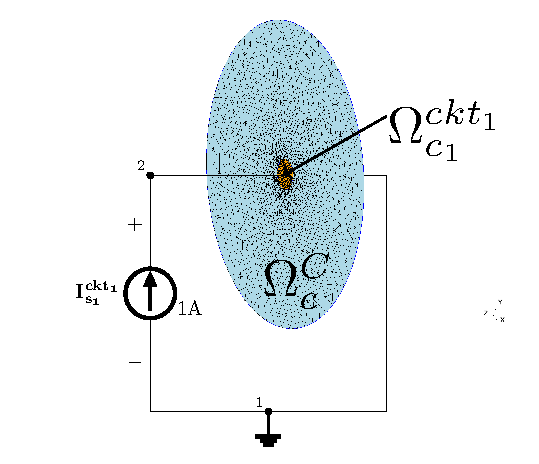
\includegraphics[width=0.5\textwidth]{current_source_sch_mesh.pdf}
\caption{Single DC current source connected to FEM Round Wire }\label{fg:dc_current_source_mesh}
\end{figure}  

To find model in our Github repository click on \href{https://github.com/ElmerCSC/elmer-elmag/tree/main/CircuitBuilder/current_source}{\textcolor{blue}{\textbf{Current Source}}}

\subsection*{Tutorial Goals}

After completing this tutorial the user will be able to:
\begin{itemize}
  \item Setup an ideal current source using the Circuit Builder, and understand the methodology behind setting up circuit equations.
  \item Understand what a Massive coil is.
  \item Run 2D  coil models in Transient and Frequency Domain.
  \item Post-process local and global quantities
  
\end{itemize}





%\subsection*{ElmerGUI Equation Menu}
\subsection*{Circuit Builder:  Ideal current source connected to 2D massive conductor}

The circuit schematics is shown in figure\ref{fg:dc_current_source}.


\begin{figure}[H]
\centering
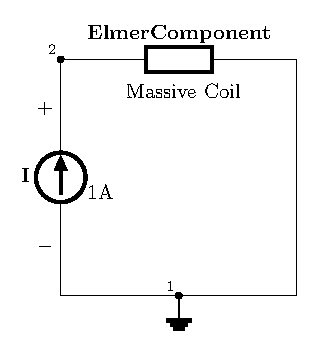
\includegraphics[width=0.35\textwidth]{current_source_sch.pdf}
\caption{DC current source connected to FEM Component Schematics}\label{fg:dc_current_source}
\end{figure}  



To define the source circuit we use the \textbf{Circuit Builder} , which follows the nodal circuit analysis approach to build the circuit equations of the type

\begin{equation}
  Bx = f
\end{equation}

where, B is the stiffness matrix of the system containing the Kirchhoff laws and component voltage and current information, and  f is the source term.

Following the schematics in \ref{fg:dc_current_source} we apply the following steps in the Circuit Builder

\begin{itemize}
  \item Enter file output name with .definition extension. This file includes all the circuit information needed by Elmer's input file (.sif)
  \begin{figure}[H]
\centering
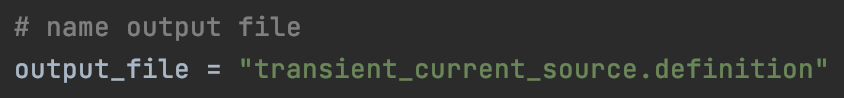
\includegraphics[width=0.7\textwidth]{T1_file.png}
%\caption{DC current source connected to FEM Component Schematics}%\label{fg:dc_current_source}
\end{figure}  
    \item Enter number of circuits in definition
      \begin{figure}[H]
\centering
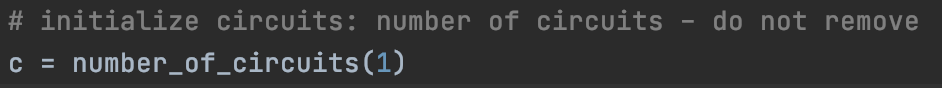
\includegraphics[width=0.7\textwidth]{T1_nckts.png}
%\caption{DC current source connected to FEM Component Schematics}%\label{fg:dc_current_source}
\end{figure}  
    \item Enter the reference node number belonging to the given circuit  
      \begin{figure}[H]
\centering
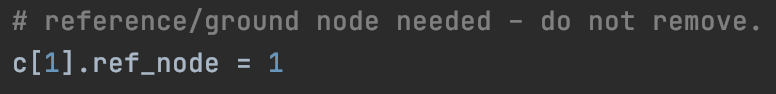
\includegraphics[width=0.7\textwidth]{T1_refnode.png}
%\caption{DC current source connected to FEM Component Schematics}%\label{fg:dc_current_source}
\end{figure}  
    \item Setup circuit components and populate given circuit with them
      \begin{figure}[H]
\centering
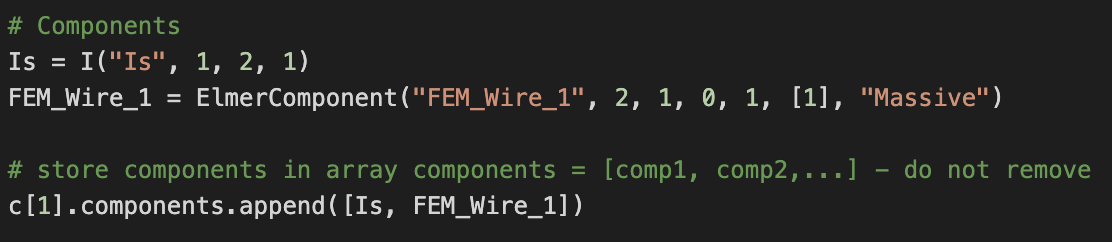
\includegraphics[width=0.8\textwidth]{T1_components.png}
%\caption{DC current source connected to FEM Component Schematics}%\label{fg:dc_current_source}
\end{figure}  

      \begin{figure}[H]
\centering
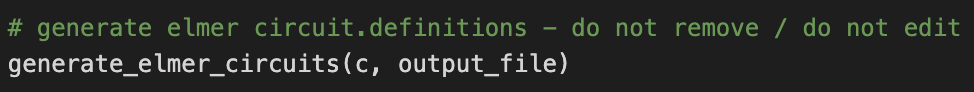
\includegraphics[width=0.8\textwidth]{T1_build_ckt.png}
%\caption{DC current source connected to FEM Component Schematics}%\label{fg:dc_current_source}
\end{figure}  

\end{itemize}



\subsection*{Pre-processing with ElmerGUI}



\begin{verbatim}
File
  Definitions
    Append -> zzz.xml
  Close
\end{verbatim}

\noindent The \texttt{\Idx{zzz.xml}} definition file is, by default, located in Linux in:

\texttt{\$ELMER\_HOME/share/ElmerGUI/edf-extra}

\noindent and in Windows, located in:

\texttt{C:/Program Files/Elmer 9.0-Release/share/ElmerGUI/edf-extra}\\

We will also be using the \Idx{zzz Solver}, which is one of the default, pre-loaded GUI definitions, so it does not need to be manually activated.  For reference, the  \texttt{\Idx{zzz.xml}} definition file is, by default, located in Linux in:

\texttt{\$ELMER\_HOME/share/ElmerGUI/edf}

\noindent and in Windows, located in:

\texttt{C:/Program Files/Elmer 9.0-Release/share/ElmerGUI/edf}\\


\subsection*{Solution procedure}

The mesh is given in ElmerGrid format in file \texttt{zzz}, load this file.

\ttbegin
File 
  Open -> zzz
\ttend



After we have the mesh we start to go through the Model menu from the top to bottom.  In the Setup we choose things related to the whole simulation such as file names, time stepping, constants etc.  

The simulation is carried out in 2-dimensional Cartesian coordinates.

zzz 2nd order bdf time stepping method is selected with zzz steps and with step size of zzz seconds.

zzz Every menu selection section must be revised for each tutorial.  These examples show the proper format and typical content.

\ttbegin
Model
  Setup 
    Simulation Type = Transient
    Steady state max. iter = 20
    Time Step Intervals = 200
    Gravity = 0 -1 0 9.82
  Apply
\ttend

In the equation section we choose the relevant equations and parameters related to their solution. 

zzz In this case we'll have one set of equations (named ``Natural Convection'') which consists of the heat equation and of the Navier-Stokes equation.

When defining Equations and Materials it is possible to assign to the bodies immediately, or to use mouse selection to assign them later. In this case we have just one body and therefore its easier to assign the Equation and Material to it directly.  It is important to select the convection to be computed since that couples the velocity field to the heat equation.

zzz The system may include non-linear iterations of each equation and steady state iterations to obtain convergence of the coupled system. It is often a good idea to keep the number of non-linear iterations in a coupled case low. Here we select just one non-linear iteration for both equations.\\

For the linear system solvers we are happy to use the defaults. One may however, try out different preconditioners (ILU1,\ldots) or direct Umfpack solver, for example.

zzz Every menu selection section must be revised for each tutorial.  These examples show the proper format and typical content.
\ttbegin
Model
  Equation
   Name = Natural Convection
    Apply to Bodies = 1
    Heat Equation
      Active = on
    Add 
    OK
\ttend        
The Material section includes all the material parameters. They are divided into generic parameters which are direct properties of the material without making any assumptions on the physical model, such as the mass. Other properties assume a physical law, such as conductivities and viscosity. 

zzz Discuss which materials are used, why they are used, and any interesting details.
   
zzz Every menu selection section must be revised for each tutorial.  These examples show the proper format and typical content.

\ttbegin
Model
  Material
    Apply to Bodies = 1 
    Material library    
      Water (room temperature)
    General 
      Reference Temperature = 293
    Add
    OK
\ttend

A Body Force represents the right-hand-side of a equation. It is generally not a required field for a body. 

zzz In this case, however, we apply the buoyancy resulting from heat expansion as a body force to the Navier-Stokes equation.

zzz Every menu selection section must be revised for each tutorial.  These examples show the proper format and typical content.

\ttbegin
Model
  Body Force
    Name = Buoyancy
    Apply to Bodies = 1
    Navier-Stokes
      Boussinesq = on
    Add 
    OK
\ttend    

Initial conditions should be given to transient cases, and probably are not needed for steady state solutions. 

zzz In this case we choose a constant Temperature field and an small initial velocity that initializes the symmetry break. 

zzz Every menu selection section must be revised for each tutorial.  These examples show the proper format and typical content.

\ttbegin
Model
  Initial Condition 
    Name = Initial Guess
    Heat Equation
      Temperature = 293
    Navier-Stokes
      Velocity 1 = 1.0e-9
      Velocity 2 = 0.0
\ttend

Only one boundary condition may be applied to each boundary and therefore all the different physical BCs for a boundary should be grouped together. 

zzz In this case the Temperature and Velocity. The side walls are assumed to be adiabatic.

zzz Every menu selection section must be revised for each tutorial.  These examples show the proper format and typical content.

\ttbegin
Model
  BoundaryCondition
    Name = Bottom
    Heat Equation
      Temperature = 293.5
    Navier-Stokes 
      Velocity 1 = 0.0
      Velocity 2 = 0.0
    Add
    New

    Name = Top
    Heat Equation
      Temperature = 293
    Navier-Stokes 
      Velocity 1 = 0.0
      Velocity 2 = 0.0
    Add
   OK 
\ttend   

The conditions may also be assigned to boundaries in the Boundary condition menu, or by clicking on each boundary with the mouse. Here we use the latter approach as that spares us of the need to know the indexes of each boundary.

zzz Every menu selection section must be revised for each tutorial.  These examples show the proper format and typical content.

\ttbegin
Model
  Set boundary properties
    Choose Bottom -> set boundary condition Bottom
    Choose Top -> set boundary condition Top
    Choose Sides -> set boundary condition Sides
   OK 
\ttend

For the execution ElmerSolver needs the mesh files and the command file.  We have now basically defined all the information for ElmerGUI to write the command file. After writing it we may also visually inspect the command file.
\ttbegin
Sif 
  Generate
  Edit -> look how your command file came out  
\ttend

Before we can execute the solver we should save the files in a directory.  The ElmerGUI project includes all the files needed to restart the case.

\ttbegin
File 
  Save Project
\ttend

After we have successfully saved the files we may start the solver.

\ttbegin
Run
  Start solver
\ttend

A convergence view automatically pops up showing relative changes of each iteration.

When there are some results to view we may start the postprocessor also.

\ttbegin
Run
  Start ParaView
\ttend

\subsection*{Results}

Due to the number of the time steps the simulation may take around zzz minutes.\\

You may inspect the results with Paraview or with ElmerVTK.\\



\subsection*{zzz Extra task:}

zzz If you have time you may try to solve the case with different parameters.

\hfill

\chapter{Voltage source connected to a 2D massive conductor }

\modinfo{Directory}{voltage\_source}
\modinfo{Transient Solvers}{\Idx{CircuitsAndDynamics}, \Idx{MagnetoDynamics2D}}
\modinfo{Harmonic Solvers}{\Idx{CircuitsAndDynamicsHarmonic}, \Idx{MagnetoDynamics2DHarmonic}}
\modinfo{Tools}{\Idx{Circuit Builder},\Idx{ElmerGUI}}
\modinfo{Dimensions}{2D, Transient, and Harmonic}
\modinfo{Author}{Jonathan Velasco}


\subsection*{Introduction}

zzz This Template For Tutorials is designed to help make it easy to create a new tutorial using ElmerGUI.  Having an outline of a tutorial should allow for simpler development of new tutorials, and will help keep the look and feel of new tutorials in unison with existing tutorials.

zzz Anywhere you see `zzz', it means that section needs to be replaced.  Any text that begins with `zzz', should be deleted and replaced by the appropriate text for your tutorial.  

zzz Think of `zzz' as a spot where you should `fill in the blanks'.



\subsection*{Case definition}


zzz Enter your case definition here.

The geometry for this tutorial looks like as shown in figure \ref{fg:geometry}.

zzz Enter your geometry figure here.

\begin{figure}[H]
\centering
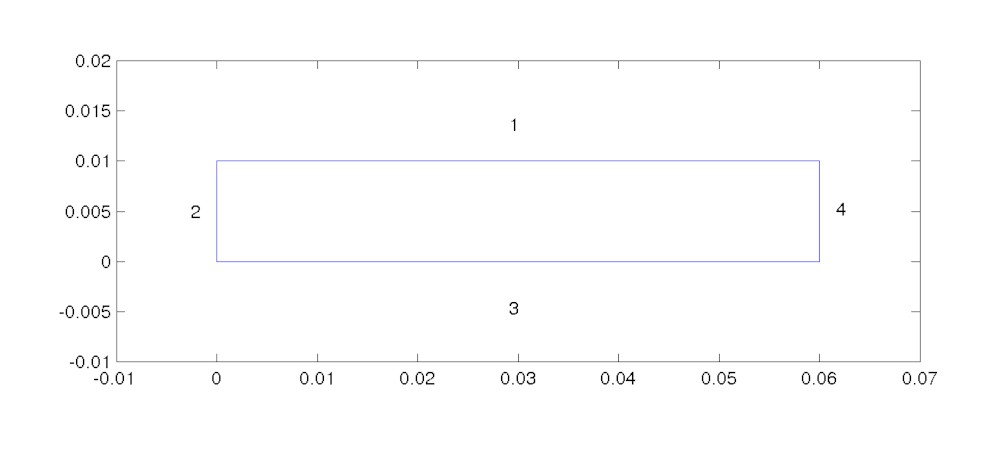
\includegraphics[width=0.8\textwidth]{geometry.png}
\caption{Geometry}\label{fg:geometry}
\end{figure}  

\subsection*{ElmerGUI Equation Menu}

zzz Note that we include both edf and edf-extra examples.  If you don't need the edf-extra example, the first section can be deleted.  It is suggested to keep the edf example, to show where the edf file comes from.

zzz The GUI definitions of zzz solver utilized in this tutorial are located in the \texttt{edf-extra} folder and thus need to be manually activated in the ElmerGUI.\\

zzz Note that the extra definition needs to be loaded first, before any other steps in building any tutorial.  Once the extra definition has been loaded, and the ElmerGUI project has been saved, then the reference to the extra definition will be stored in the project, and you won't have to load the extra definition again.

\begin{verbatim}
File
  Definitions
    Append -> zzz.xml
  Close
\end{verbatim}

\noindent The \texttt{\Idx{zzz.xml}} definition file is, by default, located in Linux in:

\texttt{\$ELMER\_HOME/share/ElmerGUI/edf-extra}

\noindent and in Windows, located in:

\texttt{C:/Program Files/Elmer 9.0-Release/share/ElmerGUI/edf-extra}\\

We will also be using the \Idx{zzz Solver}, which is one of the default, pre-loaded GUI definitions, so it does not need to be manually activated.  For reference, the  \texttt{\Idx{zzz.xml}} definition file is, by default, located in Linux in:

\texttt{\$ELMER\_HOME/share/ElmerGUI/edf}

\noindent and in Windows, located in:

\texttt{C:/Program Files/Elmer 9.0-Release/share/ElmerGUI/edf}\\


\subsection*{Solution procedure}

The mesh is given in ElmerGrid format in file \texttt{zzz}, load this file.

\ttbegin
File 
  Open -> zzz
\ttend

You should obtain your mesh and may check \texttt{Model Summary...} that it consists of zzz elements.  Your mesh should look like as shown in figure \ref{fg:mesh}

\begin{figure}[H]
\centering
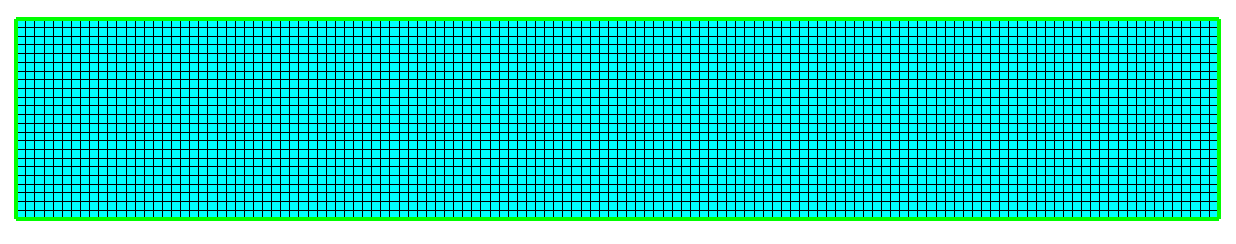
\includegraphics[width=0.8\textwidth]{mesh}
\caption{Mesh}\label{fg:mesh}
\end{figure}

After we have the mesh we start to go through the Model menu from the top to bottom.  In the Setup we choose things related to the whole simulation such as file names, time stepping, constants etc.  

The simulation is carried out in 2-dimensional Cartesian coordinates.

zzz 2nd order bdf time stepping method is selected with zzz steps and with step size of zzz seconds.

zzz Every menu selection section must be revised for each tutorial.  These examples show the proper format and typical content.

\ttbegin
Model
  Setup 
    Simulation Type = Transient
    Steady state max. iter = 20
    Time Step Intervals = 200
    Gravity = 0 -1 0 9.82
  Apply
\ttend

In the equation section we choose the relevant equations and parameters related to their solution. 

zzz In this case we'll have one set of equations (named ``Natural Convection'') which consists of the heat equation and of the Navier-Stokes equation.

When defining Equations and Materials it is possible to assign to the bodies immediately, or to use mouse selection to assign them later. In this case we have just one body and therefore its easier to assign the Equation and Material to it directly.  It is important to select the convection to be computed since that couples the velocity field to the heat equation.

zzz The system may include non-linear iterations of each equation and steady state iterations to obtain convergence of the coupled system. It is often a good idea to keep the number of non-linear iterations in a coupled case low. Here we select just one non-linear iteration for both equations.\\

For the linear system solvers we are happy to use the defaults. One may however, try out different preconditioners (ILU1,\ldots) or direct Umfpack solver, for example.

zzz Every menu selection section must be revised for each tutorial.  These examples show the proper format and typical content.
\ttbegin
Model
  Equation
   Name = Natural Convection
    Apply to Bodies = 1
    Heat Equation
      Active = on
    Add 
    OK
\ttend        
The Material section includes all the material parameters. They are divided into generic parameters which are direct properties of the material without making any assumptions on the physical model, such as the mass. Other properties assume a physical law, such as conductivities and viscosity. 

zzz Discuss which materials are used, why they are used, and any interesting details.
   
zzz Every menu selection section must be revised for each tutorial.  These examples show the proper format and typical content.

\ttbegin
Model
  Material
    Apply to Bodies = 1 
    Material library    
      Water (room temperature)
    General 
      Reference Temperature = 293
    Add
    OK
\ttend

A Body Force represents the right-hand-side of a equation. It is generally not a required field for a body. 

zzz In this case, however, we apply the buoyancy resulting from heat expansion as a body force to the Navier-Stokes equation.

zzz Every menu selection section must be revised for each tutorial.  These examples show the proper format and typical content.

\ttbegin
Model
  Body Force
    Name = Buoyancy
    Apply to Bodies = 1
    Navier-Stokes
      Boussinesq = on
    Add 
    OK
\ttend    

Initial conditions should be given to transient cases, and probably are not needed for steady state solutions. 

zzz In this case we choose a constant Temperature field and an small initial velocity that initializes the symmetry break. 

zzz Every menu selection section must be revised for each tutorial.  These examples show the proper format and typical content.

\ttbegin
Model
  Initial Condition 
    Name = Initial Guess
    Heat Equation
      Temperature = 293
    Navier-Stokes
      Velocity 1 = 1.0e-9
      Velocity 2 = 0.0
\ttend

Only one boundary condition may be applied to each boundary and therefore all the different physical BCs for a boundary should be grouped together. 

zzz In this case the Temperature and Velocity. The side walls are assumed to be adiabatic.

zzz Every menu selection section must be revised for each tutorial.  These examples show the proper format and typical content.

\ttbegin
Model
  BoundaryCondition
    Name = Bottom
    Heat Equation
      Temperature = 293.5
    Navier-Stokes 
      Velocity 1 = 0.0
      Velocity 2 = 0.0
    Add
    New

    Name = Top
    Heat Equation
      Temperature = 293
    Navier-Stokes 
      Velocity 1 = 0.0
      Velocity 2 = 0.0
    Add
   OK 
\ttend   

The conditions may also be assigned to boundaries in the Boundary condition menu, or by clicking on each boundary with the mouse. Here we use the latter approach as that spares us of the need to know the indexes of each boundary.

zzz Every menu selection section must be revised for each tutorial.  These examples show the proper format and typical content.

\ttbegin
Model
  Set boundary properties
    Choose Bottom -> set boundary condition Bottom
    Choose Top -> set boundary condition Top
    Choose Sides -> set boundary condition Sides
   OK 
\ttend

For the execution ElmerSolver needs the mesh files and the command file.  We have now basically defined all the information for ElmerGUI to write the command file. After writing it we may also visually inspect the command file.
\ttbegin
Sif 
  Generate
  Edit -> look how your command file came out  
\ttend

Before we can execute the solver we should save the files in a directory.  The ElmerGUI project includes all the files needed to restart the case.

\ttbegin
File 
  Save Project
\ttend

After we have successfully saved the files we may start the solver.

\ttbegin
Run
  Start solver
\ttend

A convergence view automatically pops up showing relative changes of each iteration.

When there are some results to view we may start the postprocessor also.

\ttbegin
Run
  Start ParaView
\ttend

\subsection*{Results}

Due to the number of the time steps the simulation may take around zzz minutes.\\

You may inspect the results with Paraview or with ElmerVTK.\\

zzz In Figure \ref{fg:temp} the obtained temperature distribution is presented. 

\begin{figure}[H]
\centering
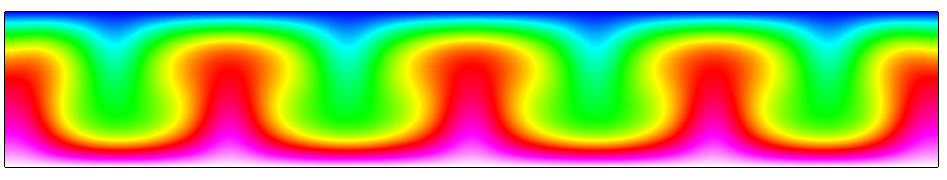
\includegraphics[width=0.8\textwidth]{temp}
\caption{zzz Temperature distribution at 260 s.}\label{fg:temp}
\end{figure} 

\subsection*{zzz Extra task:}

zzz If you have time you may try to solve the case with different parameters.

\hfill

\chapter{Voltage divider connected to a 2D stranded conductor }

\modinfo{Directory}{voltage\_source}
\modinfo{Transient Solvers}{\Idx{CircuitsAndDynamics}, \Idx{MagnetoDynamics2D}}
\modinfo{Harmonic Solvers}{\Idx{CircuitsAndDynamicsHarmonic}, \Idx{MagnetoDynamics2DHarmonic}}
\modinfo{Tools}{\Idx{Circuit Builder},\Idx{ElmerGUI}}
\modinfo{Dimensions}{2D, Transient, and Harmonic}
\modinfo{Author}{Jonathan Velasco}


\subsection*{Introduction}

zzz This Template For Tutorials is designed to help make it easy to create a new tutorial using ElmerGUI.  Having an outline of a tutorial should allow for simpler development of new tutorials, and will help keep the look and feel of new tutorials in unison with existing tutorials.

zzz Anywhere you see `zzz', it means that section needs to be replaced.  Any text that begins with `zzz', should be deleted and replaced by the appropriate text for your tutorial.  

zzz Think of `zzz' as a spot where you should `fill in the blanks'.

\begin{figure}[H]
\centering
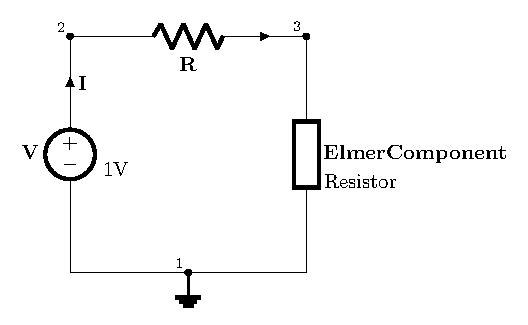
\includegraphics[width=0.35\textwidth]{voltage_divider_sch.pdf}
\caption{Voltage divider with a lumped resistor and FEM "resistor" component Schematics}\label{fg:dc_voltage_divider}
\end{figure}  

\subsection*{Case definition}


zzz Enter your case definition here.

The geometry for this tutorial looks like as shown in figure \ref{fg:geometry}.

zzz Enter your geometry figure here.

\begin{figure}[H]
\centering
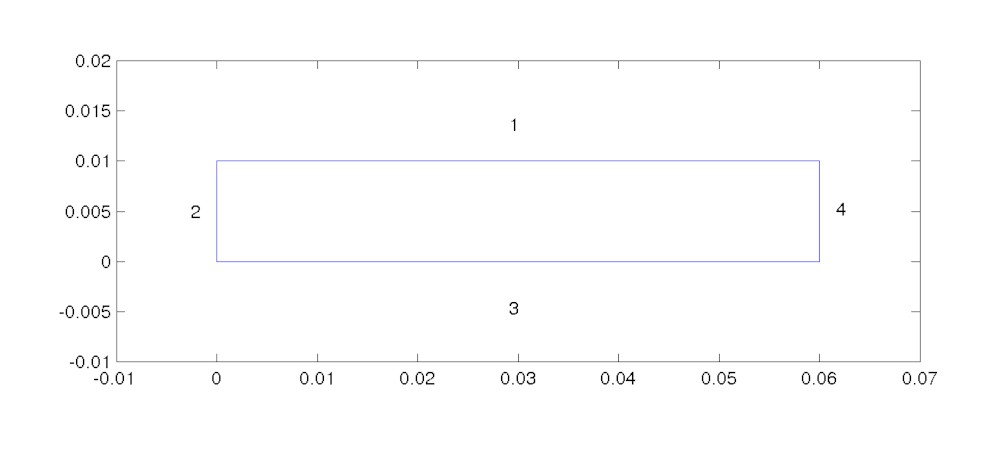
\includegraphics[width=0.8\textwidth]{geometry.png}
\caption{Geometry}\label{fg:geometry}
\end{figure}  

\subsection*{ElmerGUI Equation Menu}

zzz Note that we include both edf and edf-extra examples.  If you don't need the edf-extra example, the first section can be deleted.  It is suggested to keep the edf example, to show where the edf file comes from.

zzz The GUI definitions of zzz solver utilized in this tutorial are located in the \texttt{edf-extra} folder and thus need to be manually activated in the ElmerGUI.\\

zzz Note that the extra definition needs to be loaded first, before any other steps in building any tutorial.  Once the extra definition has been loaded, and the ElmerGUI project has been saved, then the reference to the extra definition will be stored in the project, and you won't have to load the extra definition again.

\begin{verbatim}
File
  Definitions
    Append -> zzz.xml
  Close
\end{verbatim}

\noindent The \texttt{\Idx{zzz.xml}} definition file is, by default, located in Linux in:

\texttt{\$ELMER\_HOME/share/ElmerGUI/edf-extra}

\noindent and in Windows, located in:

\texttt{C:/Program Files/Elmer 9.0-Release/share/ElmerGUI/edf-extra}\\

We will also be using the \Idx{zzz Solver}, which is one of the default, pre-loaded GUI definitions, so it does not need to be manually activated.  For reference, the  \texttt{\Idx{zzz.xml}} definition file is, by default, located in Linux in:

\texttt{\$ELMER\_HOME/share/ElmerGUI/edf}

\noindent and in Windows, located in:

\texttt{C:/Program Files/Elmer 9.0-Release/share/ElmerGUI/edf}\\


\subsection*{Solution procedure}

The mesh is given in ElmerGrid format in file \texttt{zzz}, load this file.

\ttbegin
File 
  Open -> zzz
\ttend

You should obtain your mesh and may check \texttt{Model Summary...} that it consists of zzz elements.  Your mesh should look like as shown in figure \ref{fg:mesh}

\begin{figure}[H]
\centering
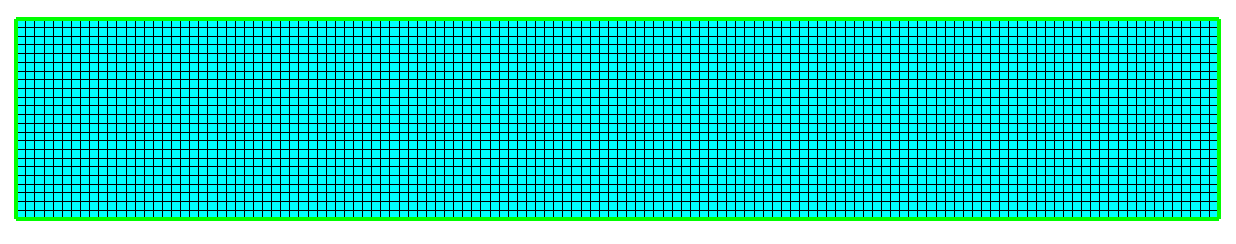
\includegraphics[width=0.8\textwidth]{mesh}
\caption{Mesh}\label{fg:mesh}
\end{figure}

After we have the mesh we start to go through the Model menu from the top to bottom.  In the Setup we choose things related to the whole simulation such as file names, time stepping, constants etc.  

The simulation is carried out in 2-dimensional Cartesian coordinates.

zzz 2nd order bdf time stepping method is selected with zzz steps and with step size of zzz seconds.

zzz Every menu selection section must be revised for each tutorial.  These examples show the proper format and typical content.

\ttbegin
Model
  Setup 
    Simulation Type = Transient
    Steady state max. iter = 20
    Time Step Intervals = 200
    Gravity = 0 -1 0 9.82
  Apply
\ttend

In the equation section we choose the relevant equations and parameters related to their solution. 

zzz In this case we'll have one set of equations (named ``Natural Convection'') which consists of the heat equation and of the Navier-Stokes equation.

When defining Equations and Materials it is possible to assign to the bodies immediately, or to use mouse selection to assign them later. In this case we have just one body and therefore its easier to assign the Equation and Material to it directly.  It is important to select the convection to be computed since that couples the velocity field to the heat equation.

zzz The system may include non-linear iterations of each equation and steady state iterations to obtain convergence of the coupled system. It is often a good idea to keep the number of non-linear iterations in a coupled case low. Here we select just one non-linear iteration for both equations.\\

For the linear system solvers we are happy to use the defaults. One may however, try out different preconditioners (ILU1,\ldots) or direct Umfpack solver, for example.

zzz Every menu selection section must be revised for each tutorial.  These examples show the proper format and typical content.
\ttbegin
Model
  Equation
   Name = Natural Convection
    Apply to Bodies = 1
    Heat Equation
      Active = on
    Add 
    OK
\ttend        
The Material section includes all the material parameters. They are divided into generic parameters which are direct properties of the material without making any assumptions on the physical model, such as the mass. Other properties assume a physical law, such as conductivities and viscosity. 

zzz Discuss which materials are used, why they are used, and any interesting details.
   
zzz Every menu selection section must be revised for each tutorial.  These examples show the proper format and typical content.

\ttbegin
Model
  Material
    Apply to Bodies = 1 
    Material library    
      Water (room temperature)
    General 
      Reference Temperature = 293
    Add
    OK
\ttend

A Body Force represents the right-hand-side of a equation. It is generally not a required field for a body. 

zzz In this case, however, we apply the buoyancy resulting from heat expansion as a body force to the Navier-Stokes equation.

zzz Every menu selection section must be revised for each tutorial.  These examples show the proper format and typical content.

\ttbegin
Model
  Body Force
    Name = Buoyancy
    Apply to Bodies = 1
    Navier-Stokes
      Boussinesq = on
    Add 
    OK
\ttend    

Initial conditions should be given to transient cases, and probably are not needed for steady state solutions. 

zzz In this case we choose a constant Temperature field and an small initial velocity that initializes the symmetry break. 

zzz Every menu selection section must be revised for each tutorial.  These examples show the proper format and typical content.

\ttbegin
Model
  Initial Condition 
    Name = Initial Guess
    Heat Equation
      Temperature = 293
    Navier-Stokes
      Velocity 1 = 1.0e-9
      Velocity 2 = 0.0
\ttend

Only one boundary condition may be applied to each boundary and therefore all the different physical BCs for a boundary should be grouped together. 

zzz In this case the Temperature and Velocity. The side walls are assumed to be adiabatic.

zzz Every menu selection section must be revised for each tutorial.  These examples show the proper format and typical content.

\ttbegin
Model
  BoundaryCondition
    Name = Bottom
    Heat Equation
      Temperature = 293.5
    Navier-Stokes 
      Velocity 1 = 0.0
      Velocity 2 = 0.0
    Add
    New

    Name = Top
    Heat Equation
      Temperature = 293
    Navier-Stokes 
      Velocity 1 = 0.0
      Velocity 2 = 0.0
    Add
   OK 
\ttend   

The conditions may also be assigned to boundaries in the Boundary condition menu, or by clicking on each boundary with the mouse. Here we use the latter approach as that spares us of the need to know the indexes of each boundary.

zzz Every menu selection section must be revised for each tutorial.  These examples show the proper format and typical content.

\ttbegin
Model
  Set boundary properties
    Choose Bottom -> set boundary condition Bottom
    Choose Top -> set boundary condition Top
    Choose Sides -> set boundary condition Sides
   OK 
\ttend

For the execution ElmerSolver needs the mesh files and the command file.  We have now basically defined all the information for ElmerGUI to write the command file. After writing it we may also visually inspect the command file.
\ttbegin
Sif 
  Generate
  Edit -> look how your command file came out  
\ttend

Before we can execute the solver we should save the files in a directory.  The ElmerGUI project includes all the files needed to restart the case.

\ttbegin
File 
  Save Project
\ttend

After we have successfully saved the files we may start the solver.

\ttbegin
Run
  Start solver
\ttend

A convergence view automatically pops up showing relative changes of each iteration.

When there are some results to view we may start the postprocessor also.

\ttbegin
Run
  Start ParaView
\ttend

\subsection*{Results}

Due to the number of the time steps the simulation may take around zzz minutes.\\

You may inspect the results with Paraview or with ElmerVTK.\\

zzz In Figure \ref{fg:temp} the obtained temperature distribution is presented. 

\begin{figure}[H]
\centering
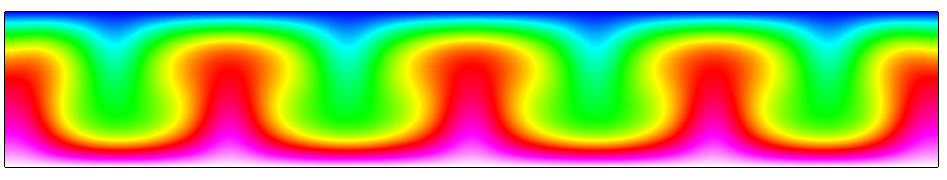
\includegraphics[width=0.8\textwidth]{temp}
\caption{zzz Temperature distribution at 260 s.}\label{fg:temp}
\end{figure} 

\subsection*{zzz Extra task:}

zzz If you have time you may try to solve the case with different parameters.

\hfill

\chapter{Current divider connected to a 2D stranded conductor }

\modinfo{Directory}{voltage\_source}
\modinfo{Transient Solvers}{\Idx{CircuitsAndDynamics}, \Idx{MagnetoDynamics2D}}
\modinfo{Harmonic Solvers}{\Idx{CircuitsAndDynamicsHarmonic}, \Idx{MagnetoDynamics2DHarmonic}}
\modinfo{Tools}{\Idx{Circuit Builder},\Idx{ElmerGUI}}
\modinfo{Dimensions}{2D, Transient, and Harmonic}
\modinfo{Author}{Jonathan Velasco}


\subsection*{Introduction}

zzz This Template For Tutorials is designed to help make it easy to create a new tutorial using ElmerGUI.  Having an outline of a tutorial should allow for simpler development of new tutorials, and will help keep the look and feel of new tutorials in unison with existing tutorials.

zzz Anywhere you see `zzz', it means that section needs to be replaced.  Any text that begins with `zzz', should be deleted and replaced by the appropriate text for your tutorial.  

zzz Think of `zzz' as a spot where you should `fill in the blanks'.

\begin{figure}[H]
\centering
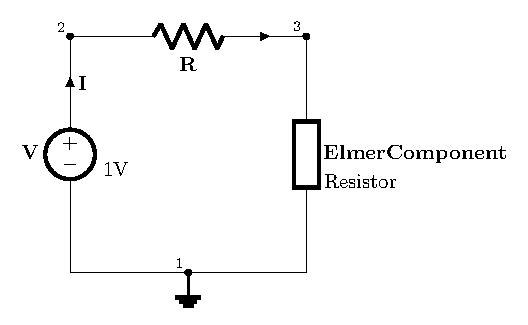
\includegraphics[width=0.35\textwidth]{voltage_divider_sch.pdf}
\caption{Current divider with a lumped resistor and FEM "resistor" component Schematics}\label{fg:dc_current_divider}
\end{figure}  

\subsection*{Case definition}


zzz Enter your case definition here.

The geometry for this tutorial looks like as shown in figure \ref{fg:geometry}.

zzz Enter your geometry figure here.

\begin{figure}[H]
\centering
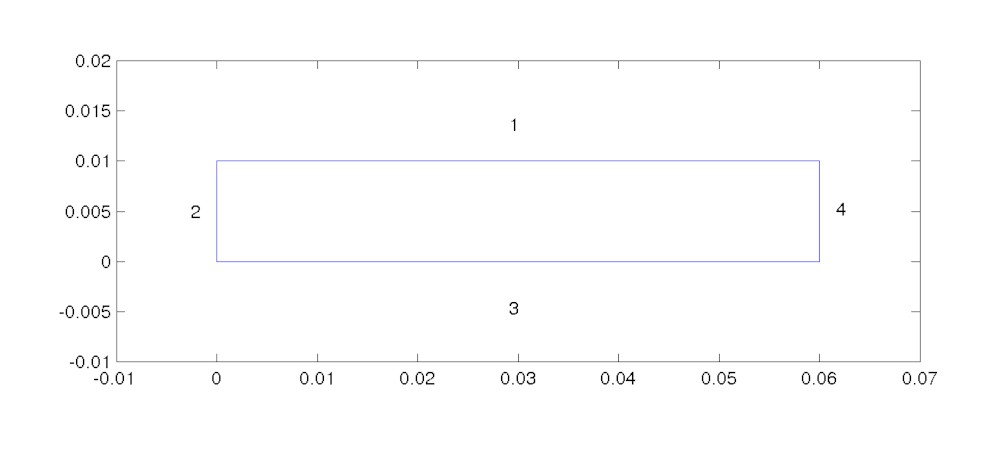
\includegraphics[width=0.8\textwidth]{geometry.png}
\caption{Geometry}\label{fg:geometry}
\end{figure}  

\subsection*{ElmerGUI Equation Menu}

zzz Note that we include both edf and edf-extra examples.  If you don't need the edf-extra example, the first section can be deleted.  It is suggested to keep the edf example, to show where the edf file comes from.

zzz The GUI definitions of zzz solver utilized in this tutorial are located in the \texttt{edf-extra} folder and thus need to be manually activated in the ElmerGUI.\\

zzz Note that the extra definition needs to be loaded first, before any other steps in building any tutorial.  Once the extra definition has been loaded, and the ElmerGUI project has been saved, then the reference to the extra definition will be stored in the project, and you won't have to load the extra definition again.

\begin{verbatim}
File
  Definitions
    Append -> zzz.xml
  Close
\end{verbatim}

\noindent The \texttt{\Idx{zzz.xml}} definition file is, by default, located in Linux in:

\texttt{\$ELMER\_HOME/share/ElmerGUI/edf-extra}

\noindent and in Windows, located in:

\texttt{C:/Program Files/Elmer 9.0-Release/share/ElmerGUI/edf-extra}\\

We will also be using the \Idx{zzz Solver}, which is one of the default, pre-loaded GUI definitions, so it does not need to be manually activated.  For reference, the  \texttt{\Idx{zzz.xml}} definition file is, by default, located in Linux in:

\texttt{\$ELMER\_HOME/share/ElmerGUI/edf}

\noindent and in Windows, located in:

\texttt{C:/Program Files/Elmer 9.0-Release/share/ElmerGUI/edf}\\


\subsection*{Solution procedure}

The mesh is given in ElmerGrid format in file \texttt{zzz}, load this file.

\ttbegin
File 
  Open -> zzz
\ttend

You should obtain your mesh and may check \texttt{Model Summary...} that it consists of zzz elements.  Your mesh should look like as shown in figure \ref{fg:mesh}

\begin{figure}[H]
\centering
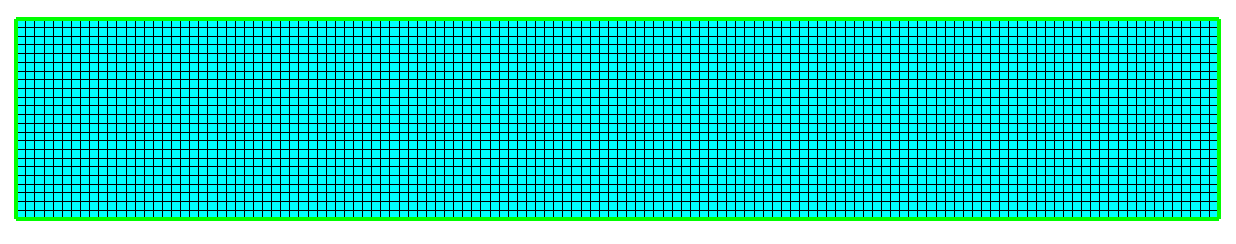
\includegraphics[width=0.8\textwidth]{mesh}
\caption{Mesh}\label{fg:mesh}
\end{figure}

After we have the mesh we start to go through the Model menu from the top to bottom.  In the Setup we choose things related to the whole simulation such as file names, time stepping, constants etc.  

The simulation is carried out in 2-dimensional Cartesian coordinates.

zzz 2nd order bdf time stepping method is selected with zzz steps and with step size of zzz seconds.

zzz Every menu selection section must be revised for each tutorial.  These examples show the proper format and typical content.

\ttbegin
Model
  Setup 
    Simulation Type = Transient
    Steady state max. iter = 20
    Time Step Intervals = 200
    Gravity = 0 -1 0 9.82
  Apply
\ttend

In the equation section we choose the relevant equations and parameters related to their solution. 

zzz In this case we'll have one set of equations (named ``Natural Convection'') which consists of the heat equation and of the Navier-Stokes equation.

When defining Equations and Materials it is possible to assign to the bodies immediately, or to use mouse selection to assign them later. In this case we have just one body and therefore its easier to assign the Equation and Material to it directly.  It is important to select the convection to be computed since that couples the velocity field to the heat equation.

zzz The system may include non-linear iterations of each equation and steady state iterations to obtain convergence of the coupled system. It is often a good idea to keep the number of non-linear iterations in a coupled case low. Here we select just one non-linear iteration for both equations.\\

For the linear system solvers we are happy to use the defaults. One may however, try out different preconditioners (ILU1,\ldots) or direct Umfpack solver, for example.

zzz Every menu selection section must be revised for each tutorial.  These examples show the proper format and typical content.
\ttbegin
Model
  Equation
   Name = Natural Convection
    Apply to Bodies = 1
    Heat Equation
      Active = on
    Add 
    OK
\ttend        
The Material section includes all the material parameters. They are divided into generic parameters which are direct properties of the material without making any assumptions on the physical model, such as the mass. Other properties assume a physical law, such as conductivities and viscosity. 

zzz Discuss which materials are used, why they are used, and any interesting details.
   
zzz Every menu selection section must be revised for each tutorial.  These examples show the proper format and typical content.

\ttbegin
Model
  Material
    Apply to Bodies = 1 
    Material library    
      Water (room temperature)
    General 
      Reference Temperature = 293
    Add
    OK
\ttend

A Body Force represents the right-hand-side of a equation. It is generally not a required field for a body. 

zzz In this case, however, we apply the buoyancy resulting from heat expansion as a body force to the Navier-Stokes equation.

zzz Every menu selection section must be revised for each tutorial.  These examples show the proper format and typical content.

\ttbegin
Model
  Body Force
    Name = Buoyancy
    Apply to Bodies = 1
    Navier-Stokes
      Boussinesq = on
    Add 
    OK
\ttend    

Initial conditions should be given to transient cases, and probably are not needed for steady state solutions. 

zzz In this case we choose a constant Temperature field and an small initial velocity that initializes the symmetry break. 

zzz Every menu selection section must be revised for each tutorial.  These examples show the proper format and typical content.

\ttbegin
Model
  Initial Condition 
    Name = Initial Guess
    Heat Equation
      Temperature = 293
    Navier-Stokes
      Velocity 1 = 1.0e-9
      Velocity 2 = 0.0
\ttend

Only one boundary condition may be applied to each boundary and therefore all the different physical BCs for a boundary should be grouped together. 

zzz In this case the Temperature and Velocity. The side walls are assumed to be adiabatic.

zzz Every menu selection section must be revised for each tutorial.  These examples show the proper format and typical content.

\ttbegin
Model
  BoundaryCondition
    Name = Bottom
    Heat Equation
      Temperature = 293.5
    Navier-Stokes 
      Velocity 1 = 0.0
      Velocity 2 = 0.0
    Add
    New

    Name = Top
    Heat Equation
      Temperature = 293
    Navier-Stokes 
      Velocity 1 = 0.0
      Velocity 2 = 0.0
    Add
   OK 
\ttend   

The conditions may also be assigned to boundaries in the Boundary condition menu, or by clicking on each boundary with the mouse. Here we use the latter approach as that spares us of the need to know the indexes of each boundary.

zzz Every menu selection section must be revised for each tutorial.  These examples show the proper format and typical content.

\ttbegin
Model
  Set boundary properties
    Choose Bottom -> set boundary condition Bottom
    Choose Top -> set boundary condition Top
    Choose Sides -> set boundary condition Sides
   OK 
\ttend

For the execution ElmerSolver needs the mesh files and the command file.  We have now basically defined all the information for ElmerGUI to write the command file. After writing it we may also visually inspect the command file.
\ttbegin
Sif 
  Generate
  Edit -> look how your command file came out  
\ttend

Before we can execute the solver we should save the files in a directory.  The ElmerGUI project includes all the files needed to restart the case.

\ttbegin
File 
  Save Project
\ttend

After we have successfully saved the files we may start the solver.

\ttbegin
Run
  Start solver
\ttend

A convergence view automatically pops up showing relative changes of each iteration.

When there are some results to view we may start the postprocessor also.

\ttbegin
Run
  Start ParaView
\ttend

\subsection*{Results}

Due to the number of the time steps the simulation may take around zzz minutes.\\

You may inspect the results with Paraview or with ElmerVTK.\\

zzz In Figure \ref{fg:temp} the obtained temperature distribution is presented. 

\begin{figure}[H]
\centering
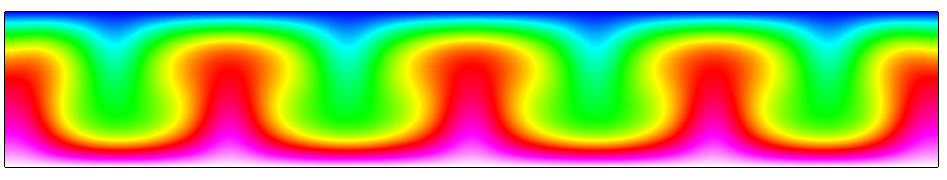
\includegraphics[width=0.8\textwidth]{temp}
\caption{zzz Temperature distribution at 260 s.}\label{fg:temp}
\end{figure} 

\subsection*{zzz Extra task:}

zzz If you have time you may try to solve the case with different parameters.

\hfill

\chapter{Three-dimensional closed-coil connected to sinusoidal current \\ TEAM Workshop Problem 7}

\modinfo{Directory}{current\_source}
\modinfo{Transient Solvers}{\Idx{CircuitsAndDynamics}, \Idx{MagnetoDynamics2D}}
\modinfo{Harmonic Solvers}{\Idx{CircuitsAndDynamicsHarmonic}, \Idx{MagnetoDynamics2DHarmonic}}
\modinfo{Tools}{\Idx{Circuit Builder}, \Idx{ElmerGUI}}
\modinfo{Dimensions}{2D}
\modinfo{Simulation Type}{Transient, and Harmonic}
\modinfo{Author}{Jonathan Velasco}


\subsection*{Introduction}

zzz This Template For Tutorials is designed to help make it easy to create a new tutorial using ElmerGUI.  Having an outline of a tutorial should allow for simpler development of new tutorials, and will help keep the look and feel of new tutorials in unison with existing tutorials.

zzz Anywhere you see `zzz', it means that section needs to be replaced.  Any text that begins with `zzz', should be deleted and replaced by the appropriate text for your tutorial.  

zzz Think of `zzz' as a spot where you should `fill in the blanks'.

\begin{figure}[H]
\centering
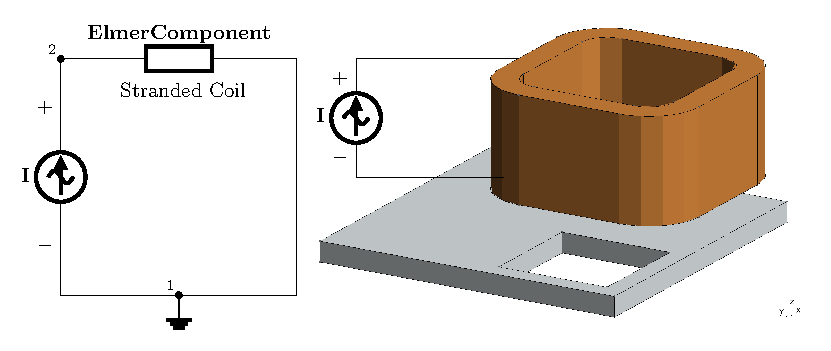
\includegraphics[width=0.8\textwidth]{TEAM7_current_source_sch.pdf}
\caption{TEAM 7 with sinusoidal current source}\label{fg:3D_coil_sinusoidal_current_source}
\end{figure}  

\subsection*{Case definition}


zzz Enter your case definition here.

The geometry for this tutorial looks like as shown in figure \ref{fg:geometry}.

zzz Enter your geometry figure here.

\begin{figure}[H]
\centering
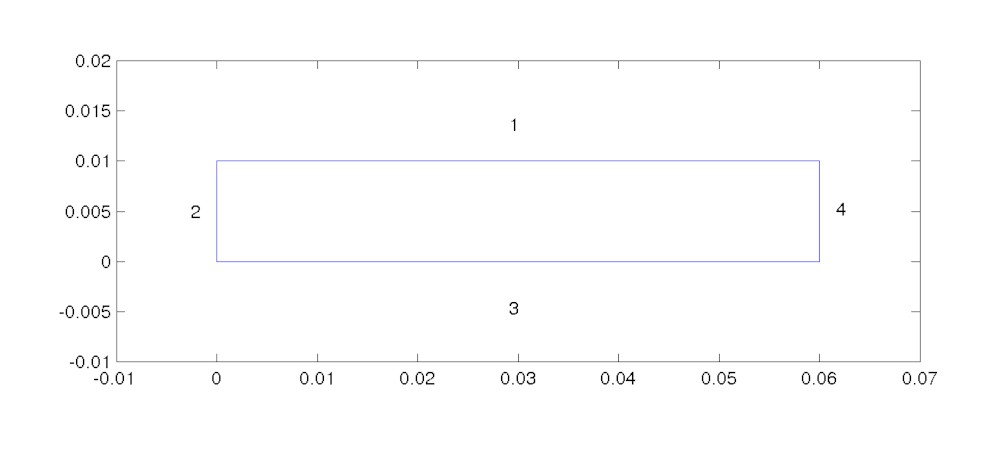
\includegraphics[width=0.8\textwidth]{geometry.png}
\caption{Geometry}\label{fg:geometry}
\end{figure}  

\subsection*{ElmerGUI Equation Menu}

zzz Note that we include both edf and edf-extra examples.  If you don't need the edf-extra example, the first section can be deleted.  It is suggested to keep the edf example, to show where the edf file comes from.

zzz The GUI definitions of zzz solver utilized in this tutorial are located in the \texttt{edf-extra} folder and thus need to be manually activated in the ElmerGUI.\\

zzz Note that the extra definition needs to be loaded first, before any other steps in building any tutorial.  Once the extra definition has been loaded, and the ElmerGUI project has been saved, then the reference to the extra definition will be stored in the project, and you won't have to load the extra definition again.

\begin{verbatim}
File
  Definitions
    Append -> zzz.xml
  Close
\end{verbatim}

\noindent The \texttt{\Idx{zzz.xml}} definition file is, by default, located in Linux in:

\texttt{\$ELMER\_HOME/share/ElmerGUI/edf-extra}

\noindent and in Windows, located in:

\texttt{C:/Program Files/Elmer 9.0-Release/share/ElmerGUI/edf-extra}\\

We will also be using the \Idx{zzz Solver}, which is one of the default, pre-loaded GUI definitions, so it does not need to be manually activated.  For reference, the  \texttt{\Idx{zzz.xml}} definition file is, by default, located in Linux in:

\texttt{\$ELMER\_HOME/share/ElmerGUI/edf}

\noindent and in Windows, located in:

\texttt{C:/Program Files/Elmer 9.0-Release/share/ElmerGUI/edf}\\


\subsection*{Solution procedure}

The mesh is given in ElmerGrid format in file \texttt{zzz}, load this file.

\ttbegin
File 
  Open -> zzz
\ttend

You should obtain your mesh and may check \texttt{Model Summary...} that it consists of zzz elements.  Your mesh should look like as shown in figure \ref{fg:mesh}

\begin{figure}[H]
\centering
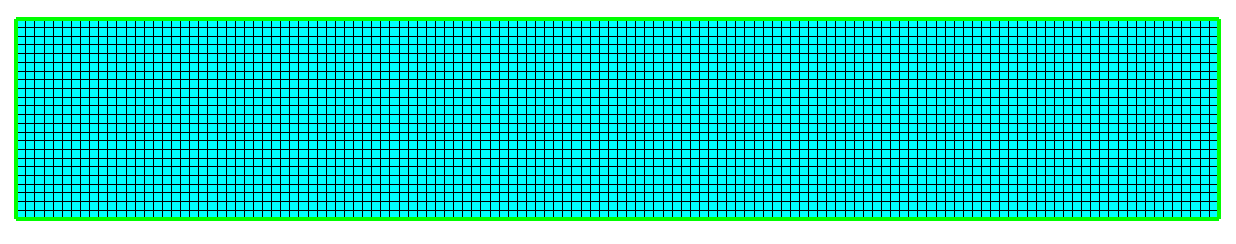
\includegraphics[width=0.8\textwidth]{mesh}
\caption{Mesh}\label{fg:mesh}
\end{figure}

After we have the mesh we start to go through the Model menu from the top to bottom.  In the Setup we choose things related to the whole simulation such as file names, time stepping, constants etc.  

The simulation is carried out in 2-dimensional Cartesian coordinates.

zzz 2nd order bdf time stepping method is selected with zzz steps and with step size of zzz seconds.

zzz Every menu selection section must be revised for each tutorial.  These examples show the proper format and typical content.

\ttbegin
Model
  Setup 
    Simulation Type = Transient
    Steady state max. iter = 20
    Time Step Intervals = 200
    Gravity = 0 -1 0 9.82
  Apply
\ttend

In the equation section we choose the relevant equations and parameters related to their solution. 

zzz In this case we'll have one set of equations (named ``Natural Convection'') which consists of the heat equation and of the Navier-Stokes equation.

When defining Equations and Materials it is possible to assign to the bodies immediately, or to use mouse selection to assign them later. In this case we have just one body and therefore its easier to assign the Equation and Material to it directly.  It is important to select the convection to be computed since that couples the velocity field to the heat equation.

zzz The system may include non-linear iterations of each equation and steady state iterations to obtain convergence of the coupled system. It is often a good idea to keep the number of non-linear iterations in a coupled case low. Here we select just one non-linear iteration for both equations.\\

For the linear system solvers we are happy to use the defaults. One may however, try out different preconditioners (ILU1,\ldots) or direct Umfpack solver, for example.

zzz Every menu selection section must be revised for each tutorial.  These examples show the proper format and typical content.
\ttbegin
Model
  Equation
   Name = Natural Convection
    Apply to Bodies = 1
    Heat Equation
      Active = on
    Add 
    OK
\ttend        
The Material section includes all the material parameters. They are divided into generic parameters which are direct properties of the material without making any assumptions on the physical model, such as the mass. Other properties assume a physical law, such as conductivities and viscosity. 

zzz Discuss which materials are used, why they are used, and any interesting details.
   
zzz Every menu selection section must be revised for each tutorial.  These examples show the proper format and typical content.

\ttbegin
Model
  Material
    Apply to Bodies = 1 
    Material library    
      Water (room temperature)
    General 
      Reference Temperature = 293
    Add
    OK
\ttend

A Body Force represents the right-hand-side of a equation. It is generally not a required field for a body. 

zzz In this case, however, we apply the buoyancy resulting from heat expansion as a body force to the Navier-Stokes equation.

zzz Every menu selection section must be revised for each tutorial.  These examples show the proper format and typical content.

\ttbegin
Model
  Body Force
    Name = Buoyancy
    Apply to Bodies = 1
    Navier-Stokes
      Boussinesq = on
    Add 
    OK
\ttend    

Initial conditions should be given to transient cases, and probably are not needed for steady state solutions. 

zzz In this case we choose a constant Temperature field and an small initial velocity that initializes the symmetry break. 

zzz Every menu selection section must be revised for each tutorial.  These examples show the proper format and typical content.

\ttbegin
Model
  Initial Condition 
    Name = Initial Guess
    Heat Equation
      Temperature = 293
    Navier-Stokes
      Velocity 1 = 1.0e-9
      Velocity 2 = 0.0
\ttend

Only one boundary condition may be applied to each boundary and therefore all the different physical BCs for a boundary should be grouped together. 

zzz In this case the Temperature and Velocity. The side walls are assumed to be adiabatic.

zzz Every menu selection section must be revised for each tutorial.  These examples show the proper format and typical content.

\ttbegin
Model
  BoundaryCondition
    Name = Bottom
    Heat Equation
      Temperature = 293.5
    Navier-Stokes 
      Velocity 1 = 0.0
      Velocity 2 = 0.0
    Add
    New

    Name = Top
    Heat Equation
      Temperature = 293
    Navier-Stokes 
      Velocity 1 = 0.0
      Velocity 2 = 0.0
    Add
   OK 
\ttend   

The conditions may also be assigned to boundaries in the Boundary condition menu, or by clicking on each boundary with the mouse. Here we use the latter approach as that spares us of the need to know the indexes of each boundary.

zzz Every menu selection section must be revised for each tutorial.  These examples show the proper format and typical content.

\ttbegin
Model
  Set boundary properties
    Choose Bottom -> set boundary condition Bottom
    Choose Top -> set boundary condition Top
    Choose Sides -> set boundary condition Sides
   OK 
\ttend

For the execution ElmerSolver needs the mesh files and the command file.  We have now basically defined all the information for ElmerGUI to write the command file. After writing it we may also visually inspect the command file.
\ttbegin
Sif 
  Generate
  Edit -> look how your command file came out  
\ttend

Before we can execute the solver we should save the files in a directory.  The ElmerGUI project includes all the files needed to restart the case.

\ttbegin
File 
  Save Project
\ttend

After we have successfully saved the files we may start the solver.

\ttbegin
Run
  Start solver
\ttend

A convergence view automatically pops up showing relative changes of each iteration.

When there are some results to view we may start the postprocessor also.

\ttbegin
Run
  Start ParaView
\ttend

\subsection*{Results}

Due to the number of the time steps the simulation may take around zzz minutes.\\

You may inspect the results with Paraview or with ElmerVTK.\\

zzz In Figure \ref{fg:temp} the obtained temperature distribution is presented. 

\begin{figure}[H]
\centering
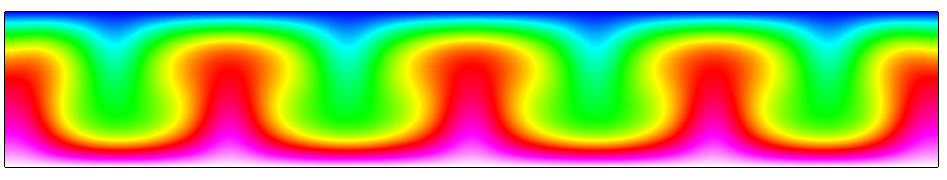
\includegraphics[width=0.8\textwidth]{temp}
\caption{zzz Temperature distribution at 260 s.}\label{fg:temp}
\end{figure} 

\subsection*{zzz Extra task:}

zzz If you have time you may try to solve the case with different parameters.

\hfill

 
 
\phantomsection % sets an anchor
\addcontentsline{toc}{part}{Index} % Include the index in TOC

\printindex


\end{document}

